%!TEX root = ../main.tex

\teaser{
	\plaatje{Voeg phong tesselation model toe.}
	
	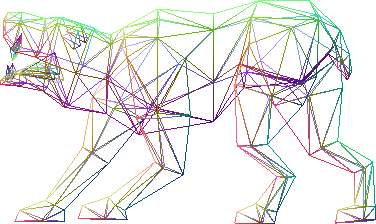
\includegraphics[width=0.3\linewidth]{content/img/header/dogWireFrame.png}
	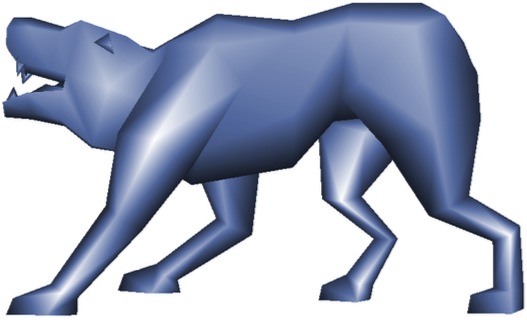
\includegraphics[width=0.3\linewidth]{content/img/header/dogModel.png}
	
\includegraphics[width=0.3\linewidth]{content/img/results/dogGPU.png}
	\centering
	\caption{From left to right: the triangular input mesh, the phong shaded mesh, and the phong shaded mesh using PN triangles and an inner and outer tessellation level of $12.0$.}
	\label{fig:preamble:teaser}
}

\maketitle